
\documentclass{article}
\usepackage{amsmath,amssymb}
\usepackage[inline]{enumitem}
\usepackage{blindtext}
\usepackage{booktabs}
\usepackage{graphicx}
\usepackage{xcolor}
\usepackage[vmargin = 1.5in, top = 1in, bottom = 1.2in, letterpaper]{geometry}
\usepackage{listings}
\usepackage{courier}
\usepackage{multicol}
\usepackage{multirow}
\usepackage{bm}
\lstset{
basicstyle = \small\tt,
keywordstyle = \tt\color{blue},
commentstyle = \it\color[cmyk]{1,0,1,0},
stringstyle = \tt\color[RGB]{128,0,0},
%frame = single,
backgroundcolor = \color[RGB]{245,245,244},
breaklines,
extendedchars = false,
xleftmargin = 2em,
xrightmargin = 2em,
aboveskip = 1em,
tabsize = 4,
showspaces = false
}
\begin{document}
\setcounter{MaxMatrixCols}{20}

% \newfontfamily\courier{Courier New}


\title{STAT 543 Homework 6}
\author{Yifan Zhu}
\maketitle

\begin{enumerate}[leftmargin = 0 em, label = \arabic*., font = \bfseries]
	\item
	$f(\bm x | \sigma_1) = \prod_{i=1}^n f(x_i | \sigma_1) = \frac{1}{(2 \pi \sigma_{1}^2)^{n/2}} \mathrm{e}^{- \frac{1}{2 \sigma_1^2} \sum_{i=1}^k x_i^2} $, we also have $f(\bm x | \sigma_0) = \prod_{i=1}^n f(x_i | \sigma_0) = \frac{1}{(2 \pi \sigma_{0}^2)^{n/2}} \mathrm{e}^{- \frac{1}{2 \sigma_0^2} \sum_{i=1}^k x_i^2}$, thus
	\begin{align*}
	&f(\bm x | \sigma_1 ) > k f(\bm x | \sigma_0)\\
	\iff & \frac{1}{(2 \pi \sigma_{1}^2)^{n/2}} \mathrm{e}^{- \frac{1}{2 \sigma_1^2} \sum_{i=1}^k x_i^2} > k \frac{1}{(2 \pi \sigma_{0}^2)^{n/2}} \mathrm{e}^{- \frac{1}{2 \sigma_0^2} \sum_{i=1}^k x_i^2} \\
	\iff & \mathrm{e}^{\left(\frac{1}{2 \sigma_0^2} - \frac{1}{2 \sigma_1^2}\right) \sum_{i=1}^n x_i^2} > k \left( \frac{\sigma_1^2}{\sigma_0^2}\right)^{n/2}\\
	\iff & \sum_{i=1}^n x_i > c,\, \textrm{because $\frac{1}{2 \sigma_{0^2}} - \frac{1}{2 \sigma_1^2} > 0$}
	\end{align*}
	Also $\sum_{i=1}^n X_i$ follows a continuous distribution, then $\gamma = 0$ and the MP test is
	\[\Phi (\bm X) = \begin{cases}
		1 & , \sum_{i=1}^n X_i > c\\
		0 & , \sum_{i=1}^n X_i < c
	\end{cases} \]

	$\alpha = E_{\sigma_0}\left( \Phi(\bm X) \right) = P_{\sigma_0}\left(\sum_{i=1}^n X_i^2 > c\right) = P_{\sigma_0}\left(\sum_{i=1}^n \left(\frac{X_i}{\sigma_0}\right)^2 > \frac{c}{\sigma_0^2}\right) = P_{\sigma_0} \left( \chi_n^2 > \frac{c}{\sigma_0^2}\right) \Rightarrow P_{\sigma_0}\left(\chi_n^2 \leq \frac{c}{\sigma_0^2}\right) = 1 - \alpha$. Hence
	\[ \frac{c}{\sigma_0^2} = \chi_{n, 1- \alpha}^2 \Rightarrow c = \sigma_0^2 \chi_{n, 1 - \alpha}^2\]


	\item 
	For every $x$, we have 

	\begin{tabular}{cccccccc}
	\toprule
		$x$ & 1 & 2 & 3 & 4 & 5 & 6 & 7\\
		\midrule
		$f(x|H_0)$ & 0.01 & 0.01 & 0.01 & 0.01 &  0.01 &0.01 & 0.94\\
		$f(x|H_1)/f(x|H_0)$ & 6 & 5 & 4 & 3 & 2 & 1 & 0.84\\
		\bottomrule
	\end{tabular}

	By Neuman-Pearson Theorem, we reject $H_0$ when $f(x|H_1)/f(x|H_0)$ is large, which corresbond to when $x$ is small. Beacause the Type I Error $\alpha = 0.04$, thus the test function is
	\[\Phi(X) = \begin{cases}
		1 & , X = 1, 2, 3, 4 \\
		0 & , otherwise
	\end{cases}\]
	And Type II Error $\beta = P_{H_1}(\Phi(X) = 0) = P_{H_1}(X = 5,6,7) = 0.82$
	\newpage
	\item 
	\begin{enumerate}
		\item 
		$\Pi_{\Phi}(\theta) = E_{\theta}(\Phi(X)) = P_{\theta}(\textrm{Reject $H_0$}) = P_{\theta} (X > 1/2) =  \int_{1/2}^1 \frac{\Gamma(\theta + 1)}{\Gamma(1) \Gamma(\theta)} x^{\theta - 1} (1 - x)^{1-1} \mathrm{d}x =1 - \left( \frac{1}{2}\right)^\theta $. The size is $\max_{\theta \in \Theta_0} \Pi_{\Phi}(\theta) = \max_{\theta \leq 1} \left\{1 - \left( \frac{1}{2}\right)^\theta\right\} = 1/2$.

		\begin{center}
		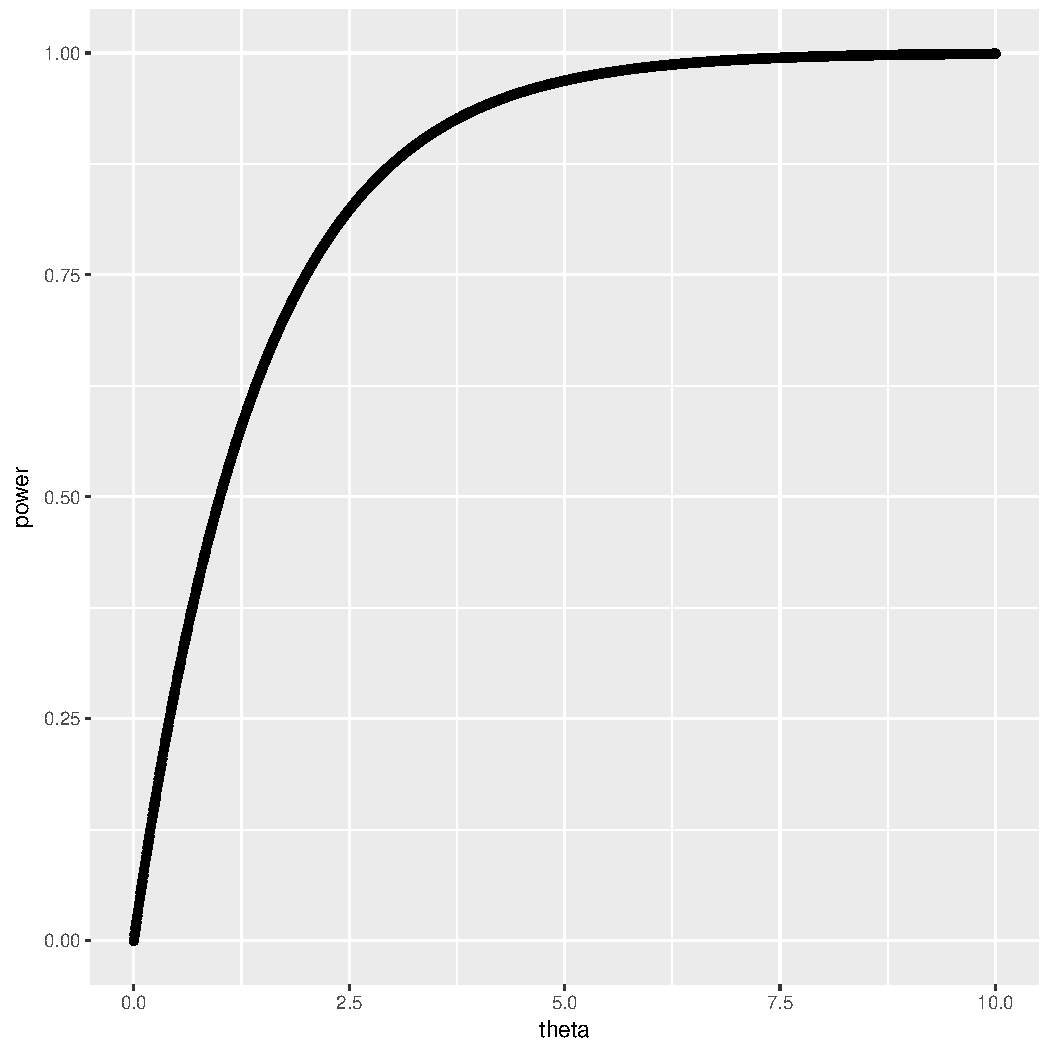
\includegraphics[width = 0.5\textwidth]{p1.pdf}
		
		\end{center}

		\item 
		$f(x | \theta) = \theta x^{\theta - 1} , f(x | 1) = 1, f(x|2) = 2x$, hence $f(x|2) > kf(x|1) \iff x > k/2$. $X$ follows a continuous distribution, then $P_{\theta_0}(X > k/2) = 1 - k/2 = \alpha \Rightarrow k /2 = 1 - \alpha$. Thus the MP test is
		\[\Phi(X) = \begin{cases}
			1 & , X > 1 - \alpha \\
			0 & , otherwise
		\end{cases}\]

		\item 
		Fix $\theta_0 \in \Theta_0$ and $\theta_1 \in \Theta_1$, we have $f(x|\theta_i) = \theta_i x^{1 - \theta_i}$. And $f(x|\theta_1) > k f(x|\theta_0) \iff \theta_1 x^{\theta_1 - 1} > k \theta_0 x^{\theta_0 - 1} \iff \frac{\theta_1}{\theta_0} x^{\theta_1 - \theta_0} > k \iff x > c$. (Because $\theta_1 > \theta_0$). Let $\max_{\theta \in \Theta_0} P_{\theta}(X > c) = \max_{\theta \in \Theta_0}\left\{\int_{c}^1 \theta x^{\theta - 1} \mathrm{d}x\right\} = \max_{\theta \in \Theta_0}\left\{1 - c^\theta\right\} = 1 - c = \alpha$. Thus $c = 1 - \alpha$ and the test function
		\[\Phi(X) = \begin{cases}
			1 & , X > 1 - \alpha\\
			0 & , otherwise
		\end{cases}\]
	\end{enumerate}
		\item 
		\begin{enumerate}
			\item 
		For any $\theta_2 > \theta_1$, 
		\[\frac{f(x|\theta_{2})}{f(x|\theta_1)} = \mathrm{e}^{\theta_1 - \theta_2} \left( \frac{1 + \mathrm{e}^{x - \theta_1}}{1 + \mathrm{e}^{x - \theta_2}}\right)\]
		And we have
		\[\frac{1 + \mathrm{e}^{x - \theta_1}}{1 + \mathrm{e}^{x - \theta_2}} = \mathrm{e}^{\theta_2 - \theta_1} + \frac{1 - \mathrm{e}^{\theta_2 - \theta_1}}{1 + \mathrm{e}^{- \theta_2} \mathrm{e}^x}\]
		$1 - \mathrm{e}^{\theta_2 - \theta_1} < 0$, thus $\left( \frac{1 + \mathrm{e}^{x - \theta_1}}{1 + \mathrm{e}^{x - \theta_2}}\right)^2 \mathrm{e}^{\theta_1 - \theta_2}$ will increase as $x$ increases. Thus it has MLR.
		\item 
		We know $\frac{f(x | 1)}{f(x | 0)}$ is increasing in $x$. Thus $\frac{f(x|1)}{f(x|0)} > k \iff x > c$. Then 
		\[P_{\theta_0}(X > c) = \int_{c}^\infty \frac{\mathrm{e}^x}{ (1 + \mathrm{e}^x)^2} \mathrm{d}x = -\frac{1}{1 + \mathrm{e}^x} \bigg |_{c}^\infty = \frac{1}{1 + \mathrm{e}^c} = \alpha \Rightarrow c = \log(1 - \alpha) - \log \alpha\]
		Thus the test function is 
		\[\Phi(X) = \begin{cases}
			1 & , X > \log (1 - \alpha) - \log \alpha\\
			0 & , otherwise
		\end{cases}\]

		For $\alpha = 0.2 \Rightarrow c = 1.386$ and Type II Error $\beta = 1 - P_{\theta_1}(X > 1.386) = 1 - \int_{1.386}^\infty \frac{\mathrm{e}^{x-1}}{(1 + \mathrm{e}^{x-1})^2} \mathrm{d}x = 1 - \int_{0.386} \frac{\mathrm{e}^t}{(1 + \mathrm{e}^{t})^2} \mathrm{d}t = 1 - \frac{1}{1 + \mathrm{e}^{0.386}} = 0.595$.

		 \item 
		  Beacause of MLR in $x$, the UMP test is the same as the MP test above.
		  \[\Phi(X) = \begin{cases}
			1 & , X > \log (1 - \alpha) - \log \alpha\\
			0 & , otherwise
		\end{cases}\]



		\item 
		$f(\bm x | \lambda) = \prod_{i=1}^n \frac{\mathrm{e}^{ - \lambda} \lambda^{x_i}}{x_i!} = \frac{\mathrm{e}^{- n \lambda} \lambda_i^{\sum_{i=1}^n x_i}}{\prod_{i=1}^n x_i!}$. Then for $\lambda_2 > \lambda_1$
		\[\frac{f(\bm x|\lambda_2)}{f(\bm x | \lambda_1)} = \frac{\mathrm{e}^{-n \lambda_2} \lambda_2 ^{\sum_{i=1}^n x_i}}{\mathrm{e}^{-n \lambda_1} \lambda_1^{\sum_{i=1}^n x_i}} = \mathrm{e}^{n(\lambda_1 - \lambda_2)} \left(\frac{\lambda_2}{\lambda_1}\right)^{\sum_{i=1}^n x_i}\]
		Hence $\frac{f(\bm x | \lambda_2)}{f(\bm x | \lambda_1)}$ increase as $\sum_{i=1}^n x_i$ increases. Thus $\{f(\bm x | \lambda): \lambda > 0\}$ have MLR in $\sum_{i=1}^n X_i$. Thus $\alpha = P_{\lambda_0}(\sum_{i=1}^n X_i > k) + \gamma P_{\lambda_0} (\sum_{i=1}^n X_i = k) \Rightarrow k = k_{n, \alpha, \lambda_0},\, \gamma = \gamma_{n, \alpha , \lambda_0}$. Then the test function is 
		\[\Phi(X) = \begin{cases}
			1 & , \sum_{i=1}^n X_i > k_{n, \alpha , \lambda_0}\\
			\gamma_{n, \alpha, \lambda_0} & , \sum_{i=1}^n X_i = k_{n, \alpha , \lambda_0}\\
			0 & , otherwise
		\end{cases}\] 

		\item 
		\begin{align*}
		P\left( \sum_{i=1}^n X_i > k \bigg| \lambda = 1 \right) = P\left(\sqrt{n}\frac{\sum_{i=1}^n (X_i - 1)}{n} > \frac{k - n}{\sqrt{n}}\bigg| \lambda = 1\right) \approx 0.05\\
		P\left( \sum_{i=1}^n X_i > k \bigg| \lambda = 2 \right) = P\left(\sqrt{n}\frac{\sum_{i=1}^n (X_i - 2)}{n} > \frac{k - 2 n}{\sqrt{2n}}\bigg| \lambda = 2\right) \approx 0.9
		\end{align*}
		Thus we have 
		\begin{align*}
		&\frac{k - n}{\sqrt{n}} = 1.645\\
		&\frac{k - 2n}{\sqrt{2n}} = -1.28
		\end{align*}
		And we can get $n = 12$ and $k = 17.7$.
		

		\end{enumerate}

		\item 
		\begin{enumerate}
			\item 
			$P(Y_n \geq 1 | \theta = 0) = 0$, then $\alpha = P(Y_1 \geq k | \theta = 0) = \int_{k}^1 n(1 - y_1)^{n-1} \mathrm{d}y_1 = (1 - k)^n$. Thus we use $k = 1 - \alpha^{1/n}$.
			\item 
			When $\theta \leq k-1$, $\Pi(\theta) = 0$.

			When $k-1 \leq \theta \leq 0$, $\Pi(\theta) = \int_{k}^{\theta + 1} n(1 - (y_1 - \theta))^{n-1} \mathrm{d}y_1 = (1 - k + \theta)^n$.

			When $0 < \theta \leq k$, $\Pi(\theta) = \int_{k}^{\theta + 1} n(1 - (y_1 - \theta))^{n-1} \mathrm{d}y_1 + \int_{\theta}^k \int_{1}^{\theta + 1} n(n-1) (y_n - y_1)^{n-2} \mathrm{d}y_n \mathrm{d}y_1 = \alpha + 1 - (1 - \theta)^n$.

			When $k < \theta$, $\Pi(\theta) = 1.$

			\item 
			\[\frac{f(\bm x | \theta)}{f(\bm x | 0)} = \frac{\bm 1 \{ \theta \leq y_1 < y_n \leq \theta + 1\}}{\bm 1\{ 0 \leq y_1 < y_n \leq 1\}}\]

			\item 
			$k = 1 - 0.1^{1/n} < 1 < \theta$, hence $\Pi(\theta) = 1$. Thus all $n = 1,2,3, \ldots$ satisfy. 
		\end{enumerate}
		
	
	

\end{enumerate}

\end{document}